\documentclass[journal,12pt,twocolumn]{IEEEtran}

\usepackage{enumitem}
\usepackage{amsmath}
\usepackage{amssymb}
\usepackage{gensymb}
\usepackage{graphicx}
\usepackage{txfonts}         
\usepackage{listings}
\usepackage{lstautogobble}
\usepackage{mathtools}
\usepackage{bm}
\usepackage{hyperref}
\usepackage{polynom}
\usepackage{capt-of}
\newcommand{\solution}{\noindent \textbf{Solution: }}
\providecommand{\pr}[1]{\ensuremath{\Pr\left(#1\right)}}
\providecommand{\brak}[1]{\ensuremath{\left(#1\right)}}
\providecommand{\cbrak}[1]{\ensuremath{\left\{#1\right\}}}
\providecommand{\sbrak}[1]{\ensuremath{\left[#1\right]}}
\providecommand{\mean}[1]{E\left[ #1 \right]}
\providecommand{\var}[1]{\mathrm{Var}\left[ #1 \right]}
\providecommand{\der}[1]{\mathrm{d} #1}
\providecommand{\gauss}[2]{\mathcal{N}\ensuremath{\left(#1,#2\right)}}
\providecommand{\mbf}{\mathbf}
\providecommand{\abs}[1]{\left\vert#1\right\vert}
\providecommand{\norm}[1]{\left\lVert#1\right\rVert}
\providecommand{\z}[1]{{\mathcal{Z}}\{#1\}}
\providecommand{\ztrans}{\overset{\mathcal{Z}}{ \rightleftharpoons}}

\providecommand{\parder}[2]{\frac{\partial}{\partial #2} \brak{#1}}

\let\StandardTheFigure\thefigure
\let\vec\mathbf

\numberwithin{equation}{section}
\renewcommand{\thefigure}{\theenumi}
\renewcommand\thesection{\arabic{section}}

\newcommand{\myvec}[1]{\ensuremath{\begin{pmatrix}#1\end{pmatrix}}}
\newcommand{\mydet}[1]{\ensuremath{\begin{vmatrix}#1\end{vmatrix}}}
\newcommand{\define}{\stackrel{\triangle}{=}}

\DeclareMathOperator*{\argmin}{arg\,min}
\DeclareMathOperator*{\argmax}{arg\,max}


\lstset {
	frame=single, 
	breaklines=true,
	columns=fullflexible,
	autogobble=true
}             
   


\begin{document}
                             
\title{ Digital Signal Processing \\ \Large EE3900: Linear Systems and Signal Processing \\ \large Indian Institute of Technology Hyderabad \\ \vspace*{12pt} \textbf{Assignment-1}}
\author{Lokesh Badisa \\ \normalsize AI21BTECH11005 \\ \vspace*{20pt} \normalsize 22 Aug 2022}   
 \maketitle 
 \begin{abstract}
 This document contains solution to Assignment-1 [ Question 3.1(f) from Discrete-Time Signal Processing by Alan V. Oppenheim and Ronald W. Schafer]
 \end{abstract}
 \section{Z-Transform}
\begin{enumerate}[label=\arabic*]
\item \textbf{[Question 3.1(f) from Discrete-Time Signal Processing by Alan V. Oppenheim] : }Determine the $z$-transform and region of convergence for the following sequence:
\begin{align}
\delta\sbrak{n+1}
\end{align}
\solution Given
\begin{align}
x(n)& = \delta\sbrak{n+1}
\end{align}
\begin{align}
\delta\sbrak{n-a}=
\begin{cases}
1 & n=a\\
0 & otherwise
\end{cases}
\end{align}
Given is Unit Sample Sequence shifted to -1.
\begin{figure}[!ht]
\begin{center}
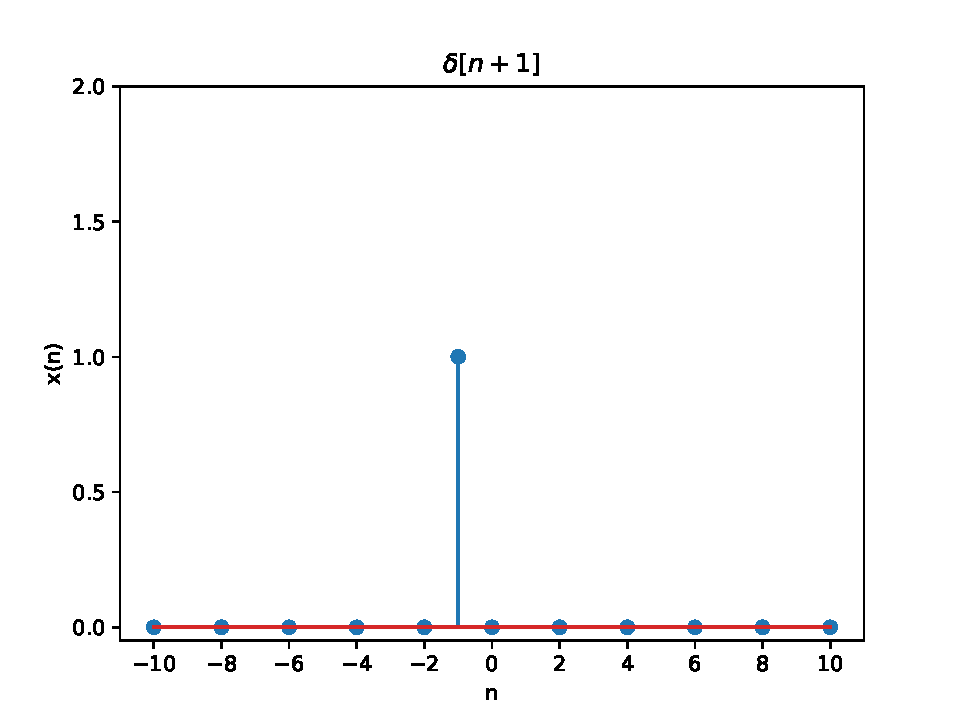
\includegraphics[width=\columnwidth]{./figs/unitsample}
\end{center}
\caption{$x(n)$}	
\end{figure}

So,
\begin{align}
\delta\sbrak{n+1}&=
\begin{cases}
1 & n=-1\\
0 & otherwise
\end{cases}\\
X(z) &= \sum_{k=-\infty}^{\infty}x(k)z^{-k}\\
&=-z
\end{align}
For $X(z)$ to converge, $\abs{X(z)}<\infty$.\\
Region of convergence:
\begin{align}
\abs{z} < \infty
\end{align}
\begin{figure}[!ht]
\begin{centering}
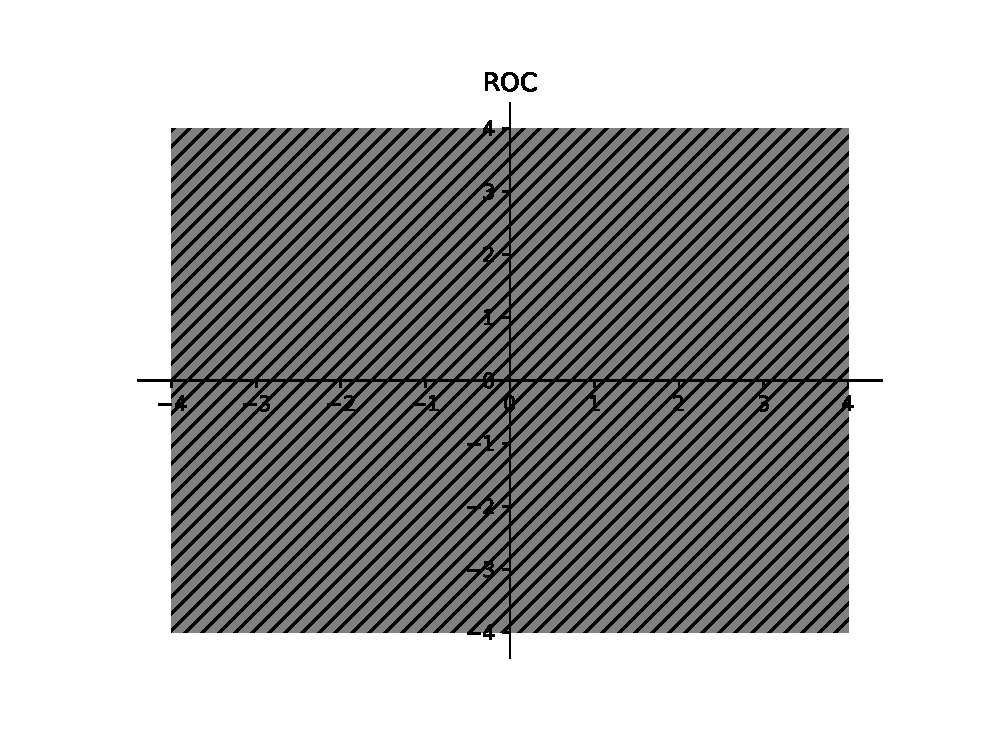
\includegraphics[width=\columnwidth]{./figs/roc}
\end{centering}
\caption{Region of Convergence}
\end{figure}
\end{enumerate} 
 \end{document}